% ============================================================
\chapter{政治と政策の不確かさ}\label{ch:politics}

戦争やテロ、選挙、関税、規制の変更は、株価を大きく動かす。調査メモは、地政学リスク指数（GPR）や経済政策不確実性指数（EPU）を使って、こうした政治のファクターを BL のビューと不確かさに変換する方法を論じている。この章では、まず指数の作り方を論文に沿って確かめ、次に BL への入れ方を 3 通りに分けて、それぞれを本プロジェクトのデータ（2015〜2026 年）で試す。

\section{地政学リスク指数（GPR）}

\begin{paperbox}[Caldara and Iacoviello（2022）, \textit{Measuring Geopolitical Risk}, American Economic Review 112(4)]
\begin{itemize}
\item \textbf{作り方}：新聞の記事のうち、悪い地政学的な出来事に触れた記事の割合を、月ごとに数える。最近の指数（1985 年から）は、アメリカ・イギリス・カナダの 10 紙（Chicago Tribune、Daily Telegraph、Financial Times、Globe and Mail、Guardian、Los Angeles Times、New York Times、USA Today、Wall Street Journal、Washington Post）の電子版を検索する。1900 年からの長い指数は、3 紙の紙面の記録を使う。
\item \textbf{検索の 8 区分}：戦争の脅威、平和への脅威、軍備の増強、核の脅威、テロの脅威（ここまで「脅威」）と、戦争の開始、戦争の激化、テロの実行（「行動」）。1 語だけの検索は誤りが多いので、2 つの語の組み合わせや、近くに現れる語で検索する。
\item \textbf{分解}：「脅威」の区分から GPRT、「行動」の区分から GPRA を作れる。
\item \textbf{確かめ方}：人が記事を読んで作った物語の記録や、さまざまな頑健性の確認で、自動の指数が意味のある動きをしていることを示す。
\item \textbf{結果}：1985〜2019 年のデータで、地政学リスクのショックは、投資と雇用の長く続く低下をもたらす。悪影響は、脅威と実際の出来事の両方から来る。
\end{itemize}
\end{paperbox}

指数は 2021 年 10 月に改訂され、検索の語が少し変わり、最近の指数は 1985〜2019 年の平均が 100 になるようにそろえられている。この資料で使ったデータ（\V{unc.start}〜\V{unc.end}）では、GPR の中央値は \V{unc.gpr.med}、最大は \V{unc.gpr.argmax} の \V{unc.gpr.max} だった。

\section{経済政策不確実性指数（EPU）}

\begin{paperbox}[Baker, Bloom and Davis（2016）, \textit{Measuring Economic Policy Uncertainty}, Quarterly Journal of Economics 131(4)]
\begin{itemize}
\item \textbf{作り方}：アメリカの主要な 10 紙（USA Today、Miami Herald、Chicago Tribune など）で、「経済」の語、「政策」の語（議会、財政赤字、連邦準備制度、立法、規制、ホワイトハウスなど）、「不確実」の語の 3 つをすべて含む記事の数を、月ごとに数える。新聞ごとに記事の総数で割り、標準化して平均し、1985〜2009 年の平均が 100 になるようにそろえる。
\item \textbf{確かめ方}：12,000 本の記事を人が読む監査を行い、自動の分類と比べた。政策の語の選び方も、この監査の結果で決めた。
\item \textbf{長い歴史}：6 紙の記録で 1900 年までさかのぼる。1931 年の終わりから大きく上がり、1960 年代から上がり続けている。
\item \textbf{結果}：接戦の大統領選挙、湾岸戦争、9.11、リーマン・ブラザーズの破綻、2011 年の債務上限の争いなどで急上昇する。企業の単位では、政策の不確実性は株価の変動を大きくし、政策に敏感な業種（防衛、医療、インフラ）の投資と雇用を減らす。
\end{itemize}
\end{paperbox}

この資料のデータでは、EPU の中央値は \V{unc.epu.med}、最大は \V{unc.epu.argmax} の \V{unc.epu.max} だった。\figref{fig:unc-series} に、EPU と GPR の内訳の推移を示す。

\begin{figure}[htbp]
\centering
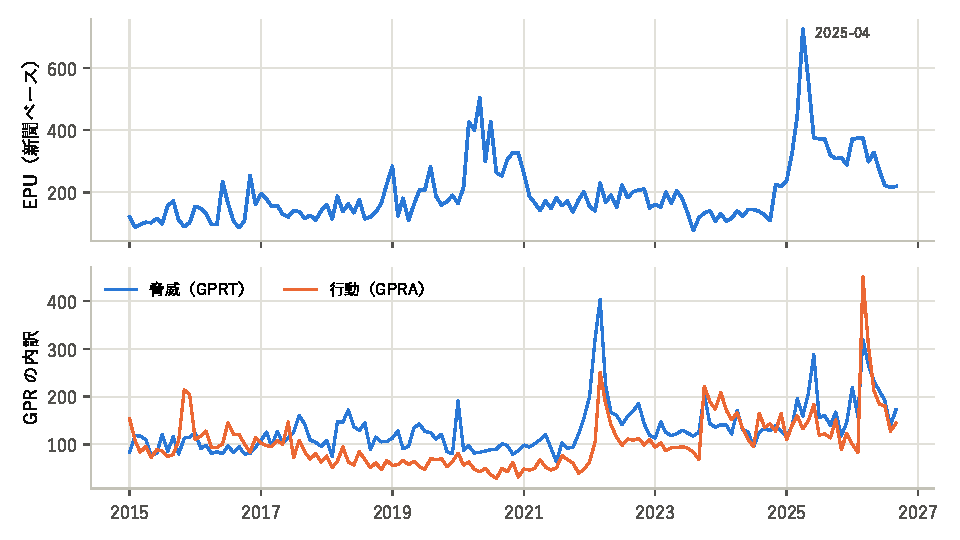
\includegraphics[width=0.95\linewidth]{fig_unc_series.pdf}
\caption{経済政策不確実性指数（上）と、地政学リスク指数の内訳（下：脅威 GPRT と行動 GPRA）。月次、\V{unc.start}〜\V{unc.end}。}
\label{fig:unc-series}
\end{figure}

\section{企業ごとの政治リスク}

\begin{paperbox}[Hassan, Hollander, van Lent and Tahoun（2019）, \textit{Firm-Level Political Risk: Measurement and Effects}, Quarterly Journal of Economics 134(4)]
\begin{itemize}
\item \textbf{作り方}：上場企業の四半期の決算説明会の書き起こしで、政治に関する話題にどれだけの時間が割かれ、それがリスクや不確実性と結びついているかを数える。政治の文章（教科書、新聞の政治面、政治の演説など）とそれ以外の文章を比べて、政治の文章に特に多い 2 語の組み合わせ（bigram）を選び、それがリスクを表す語の近くに現れる回数を数える。
\item \textbf{データ}：この資料で確かめた NBER の版では、2002〜2016 年に、アメリカで上場する 9,478 社が行った 175,797 回の決算説明会である。
\item \textbf{結果}：政治リスクの大部分は、業種や時期では説明できない企業ごとのもので、ばらつきが大きい。政治リスクが高い企業は、投資と採用を減らし、ロビー活動や献金を増やす。
\end{itemize}
\end{paperbox}

調査メモは、この方法を応用した分析として「約 7,000 社の 24 万件を超える決算説明会」から企業ごとの地政学リスクのセンチメントを取り出し、航空・運輸が悪影響を受け、防衛が恩恵を受けることを捉えた、と書いている。この資料では、その数字と結果を述べた論文を確認できなかった（\appref{app:check}）。企業ごとの政治リスクの測り方としては、上の論文が出発点になる。

\section{政治リスクは期待リターンに効くか}

政治の不確かさが、期待リターン（リスクプレミアム）とボラティリティの両方に効くことは、理論と実証の両方で論じられている。

\begin{itemize}
\item Pástor と Veronesi（2012、2013）は、政府の政策の不確かさが株価にリスクプレミアムを要求させ、ボラティリティと銘柄間の相関を高めることを、理論のモデルで示した。
\item Brogaard と Detzel（2015）は、EPU が資産価格に織り込まれたリスクの要因であることを実証し、EPU の上昇が同時点のリターンの低下と、その後のリターンの上昇（リスクプレミアム）に結びつくことを報告している。
\end{itemize}

BL の言葉に直すと、政治の不確かさが高まったときには、(1) 期待リターンの見込み（$Q$）が変わりうる、(2) リターンの散らばり（$\Sigma$）が大きくなる、(3) 予想の外れ（$\Omega$）も大きくなる、の 3 つが起きうる。以下、それぞれを順に見る。

\section{入れ方 1：感応度からビューを作る}

調査メモは、資産のリターンと GPR・EPU の時系列モデル（VAR など）を作り、ショックへの反応（インパルス応答）を測って、それをビュー $Q$ にする方法を挙げている。もっとも簡単な形は、市場のリターンを入れたうえで、指数の変化への感応度を回帰で測ることである。
\begin{equation}
r_{s,t}-r_{f,t}=a_s+\beta_{s}^{\mathrm{mkt}}(r_{m,t}-r_{f,t})+\beta_s^{\mathrm{EPU}}\Delta\log\mathrm{EPU}_t+\beta_s^{\mathrm{GPR}}\Delta\log\mathrm{GPR}_t+e_{s,t}
\end{equation}
セクター ETF の月次リターンで推定した結果を\tabref{tab:unc-sector}に示す。

\begin{table}[htbp]
\centering
\caption{セクター ETF の月次超過リターンの、EPU・GPR の変化への感応度（2015〜2026 年）。「+10\%」の列は、指数が 10\% 上がった月のリターンの違い（\%）。$t$ 値は White の標準誤差による。}
\label{tab:unc-sector}
\tabin{unc_sector}
\end{table}

感応度の $t$ 値は、ほとんどが 2 を下回る。公益は EPU と GPR の上昇月にやや強く、金融とエネルギーは EPU の上昇月にやや弱いが、偶然と区別できる大きさではない。月次で 10 年分のデータでは、セクターの政治の感応度ははっきり測れない。

仮に感応度が測れたとしても、ビューにするには「来月、指数がどう動くか」の予想が必要になる。指数の変化を予想するのは、株価を予想するのと同じくらい難しい。感応度からビューを作る方法は、次の「シナリオ」の形で使うほうが素直である。

\section{入れ方 2：シナリオとして入れる}

「もし地政学リスクが 50\% 高まったら」というシナリオを、外部の変数へのビューとして入れる（\chapref{ch:shape}）。セクターの超過リターンと指数の変化を並べた変数 $(X,g)$ の共分散を、全セクターの ETF がそろう 2018 年 7 月からの \V{scen.n} か月で推定し、市場版の BL で $g=\log1.5$（50\% の上昇）という条件を付ける。均衡のずれは 0 とした。

\begin{table}[htbp]
\centering
\caption{指数の 50\% 上昇を外部の変数へのビューとして入れたときの、セクターの期待リターンの変化（月次 \%）。「確実」は $\Omega\to0$（シナリオ分析）、「$c=1$」は $\Omega$ を指数の変化の分散と同じにしたもの。指数の月次の変化の標準偏差は、GPR が \V{scen.dgpr.sd}\%、EPU が \V{scen.depu.sd}\%。}
\label{tab:unc-scen}
\tabin{unc_scen}
\end{table}

\tabref{tab:unc-scen} のとおり、GPR が 50\% 上がるシナリオでは、公益を除く全セクターが月次で 0.5〜2\% 下がる。EPU のシナリオでは、エネルギー、金融、資本財が大きく下がり、ヘルスケアと公益はほとんど動かない。

ただし、この数字は「過去 8 年あまりの相関がこれからも続くなら」という条件付きである。GPR の変化とセクターのリターンの相関は $-0.24$〜0 と小さく、推定の誤差も大きい。シナリオの結果は、確実（$\Omega\to0$）で入れるより、$c=1$ のように控えめに入れ、ストレステストとして比率の変化を確かめる使い方が向いている。Meucci が BL の市場版を「シナリオ分析」と結びつけたのは、この使い方である。

\section{入れ方 3：不確かさ $\Omega$ を伸び縮みさせる}

調査メモがもっとも強調しているのは、政治の不確かさが高い時期に $\Omega$ を大きくして、ビューの確信度を自動的に下げる、という使い方である。

\begin{paperbox}[Han and Li（2023）, \textit{The impact of global economic policy uncertainty on portfolio optimization: A Black--Litterman approach}, International Review of Financial Analysis 86]
\begin{itemize}
\item 世界の経済政策不確実性（GEPU）が、世界の資産配分に非対称に効くことを調べる。
\item 二重に非対称な GARCH-MIDAS（DAGM）のモデルで、GEPU のショックが、世界の株式、債券、商品、クリーンエネルギー、ビットコインの長期のボラティリティに与える影響を推定する。
\item GEPU に基づくボラティリティを、BL の投資家のビューの不確かさとして使う。
\item 標本外の検証で、GEPU に基づくモデルは、多くの場合に従来の基準よりリスク調整後のリターンが高かった。
\end{itemize}
\end{paperbox}

この方法が働くには、「政治の不確かさが高い時期には、予想が外れやすい（ボラティリティが高い）」ことが必要である。本プロジェクトのデータで、月末の指数の水準が、翌月の \SP{} の実現ボラティリティ（日次リターンの標準偏差の年率）を予想できるかを調べた。

\begin{table}[htbp]
\centering
\caption{翌月の \SP{} の実現ボラティリティ（対数）の回帰（\V{unc.reg.n} か月）。説明変数は、当月の実現ボラティリティ、EPU、GPR の対数。}
\label{tab:unc-reg}
\tabin{unc_reg}
\end{table}

結果は次のとおりである。

\begin{itemize}
\item 単独の相関では、EPU は翌月のボラティリティと \V{unc.cor.epu}、GPR は \V{unc.cor.gpr} の相関を持つ。当月の実現ボラティリティは \V{unc.cor.rv}、VIX は \V{unc.cor.vix} である。
\item 当月の実現ボラティリティを入れると、EPU の $t$ 値は \V{unc.reg.epu.t}、GPR は \V{unc.reg.gpr.t} で、追加の説明力はない（\tabref{tab:unc-reg}）。
\item VIX を入れると、VIX の $t$ 値は \V{unc.reg2.vix.t} で強く、EPU は \V{unc.reg2.epu.t} とむしろ負になった。
\end{itemize}

少なくとも、翌月という短い期間では、政治の指数は市場のボラティリティ（直近の実現値や VIX）にない情報をほとんど持っていない。新聞の記事の数より、市場の価格のほうが早く、正確に不確かさを映しているためと考えられる。Han と Li の方法が長期のボラティリティの成分（MIDAS）を使っているのは、政策の不確かさが効くのは月次より長い期間だ、という見方と整合する。

それでも EPU で $\Omega$ を伸び縮みさせたらどうなるかを、\chapref{ch:macro} の\figref{fig:adoption-time}に示した。EPU の中央値で採用率 50\% になるように置くと、関税をめぐる不確実性が急上昇した 2025 年 4 月には、採用率は \V{epu.adopt.min}\% まで下がる。仕組みとしては働くが、上のとおり、その時期に予想が本当に外れやすいかの裏付けは弱い。

\section{調査メモの記述について}

調査メモは、GPR の「脅威」（GPRT）を不確かさ $\Omega$ を大きくする合図に、「行動」（GPRA）を防衛・エネルギーなどのセクターへの方向のビューに使う、という表を示している。この対応は、Caldara と Iacoviello の論文にはない。論文が示しているのは、脅威と行動の両方が実体経済に悪影響を与えることである。表は、調査メモの提案として読むのがよい。この資料のデータでは、脅威と行動の区別に入る前に、指数そのものが翌月のボラティリティやセクターの差をほとんど説明しなかった。

\begin{tipbox}[コツ：政治のファクターを使うとき]
\begin{enumerate}
\item 感応度を推定して来月のビューにするのは難しい。指数の変化そのものを予想しなければならないうえ、感応度の推定の誤差も大きい。
\item 「もし地政学リスクが高まったら」という問いには、市場版の BL のシナリオ（外部の変数へのビュー）で答える。結果はストレステストとして使い、確実なビューとして入れない。
\item $\Omega$ を伸び縮みさせるなら、まず市場のボラティリティ（直近の実現値、VIX）を使う。政治の指数は、それに加えて説明力があるかを確かめてから使う。
\item 政策の不確かさが効くのは、月次より長い期間かもしれない。期間の長いビューや、長期のボラティリティの成分と組み合わせる。
\end{enumerate}
\end{tipbox}

\begin{keybox}[この章のまとめ]
\begin{itemize}
\item GPR と EPU は、新聞の記事の割合から作る月次の指数である。企業ごとの政治リスクは、決算説明会の書き起こしから測れる（Hassan ほか 2019）。
\item 本プロジェクトのデータ（2015〜2026 年）では、セクターの感応度ははっきりせず、指数は翌月のボラティリティを市場の指標以上には説明しなかった。
\item 政治のファクターは、シナリオ分析と、長い期間の不確かさの見込みに使うのが向いている。
\end{itemize}
\end{keybox}
